\begin{figure}[t]
    \centering
    \begin{subfigure}[t]{0.19\textwidth}
        \centering
        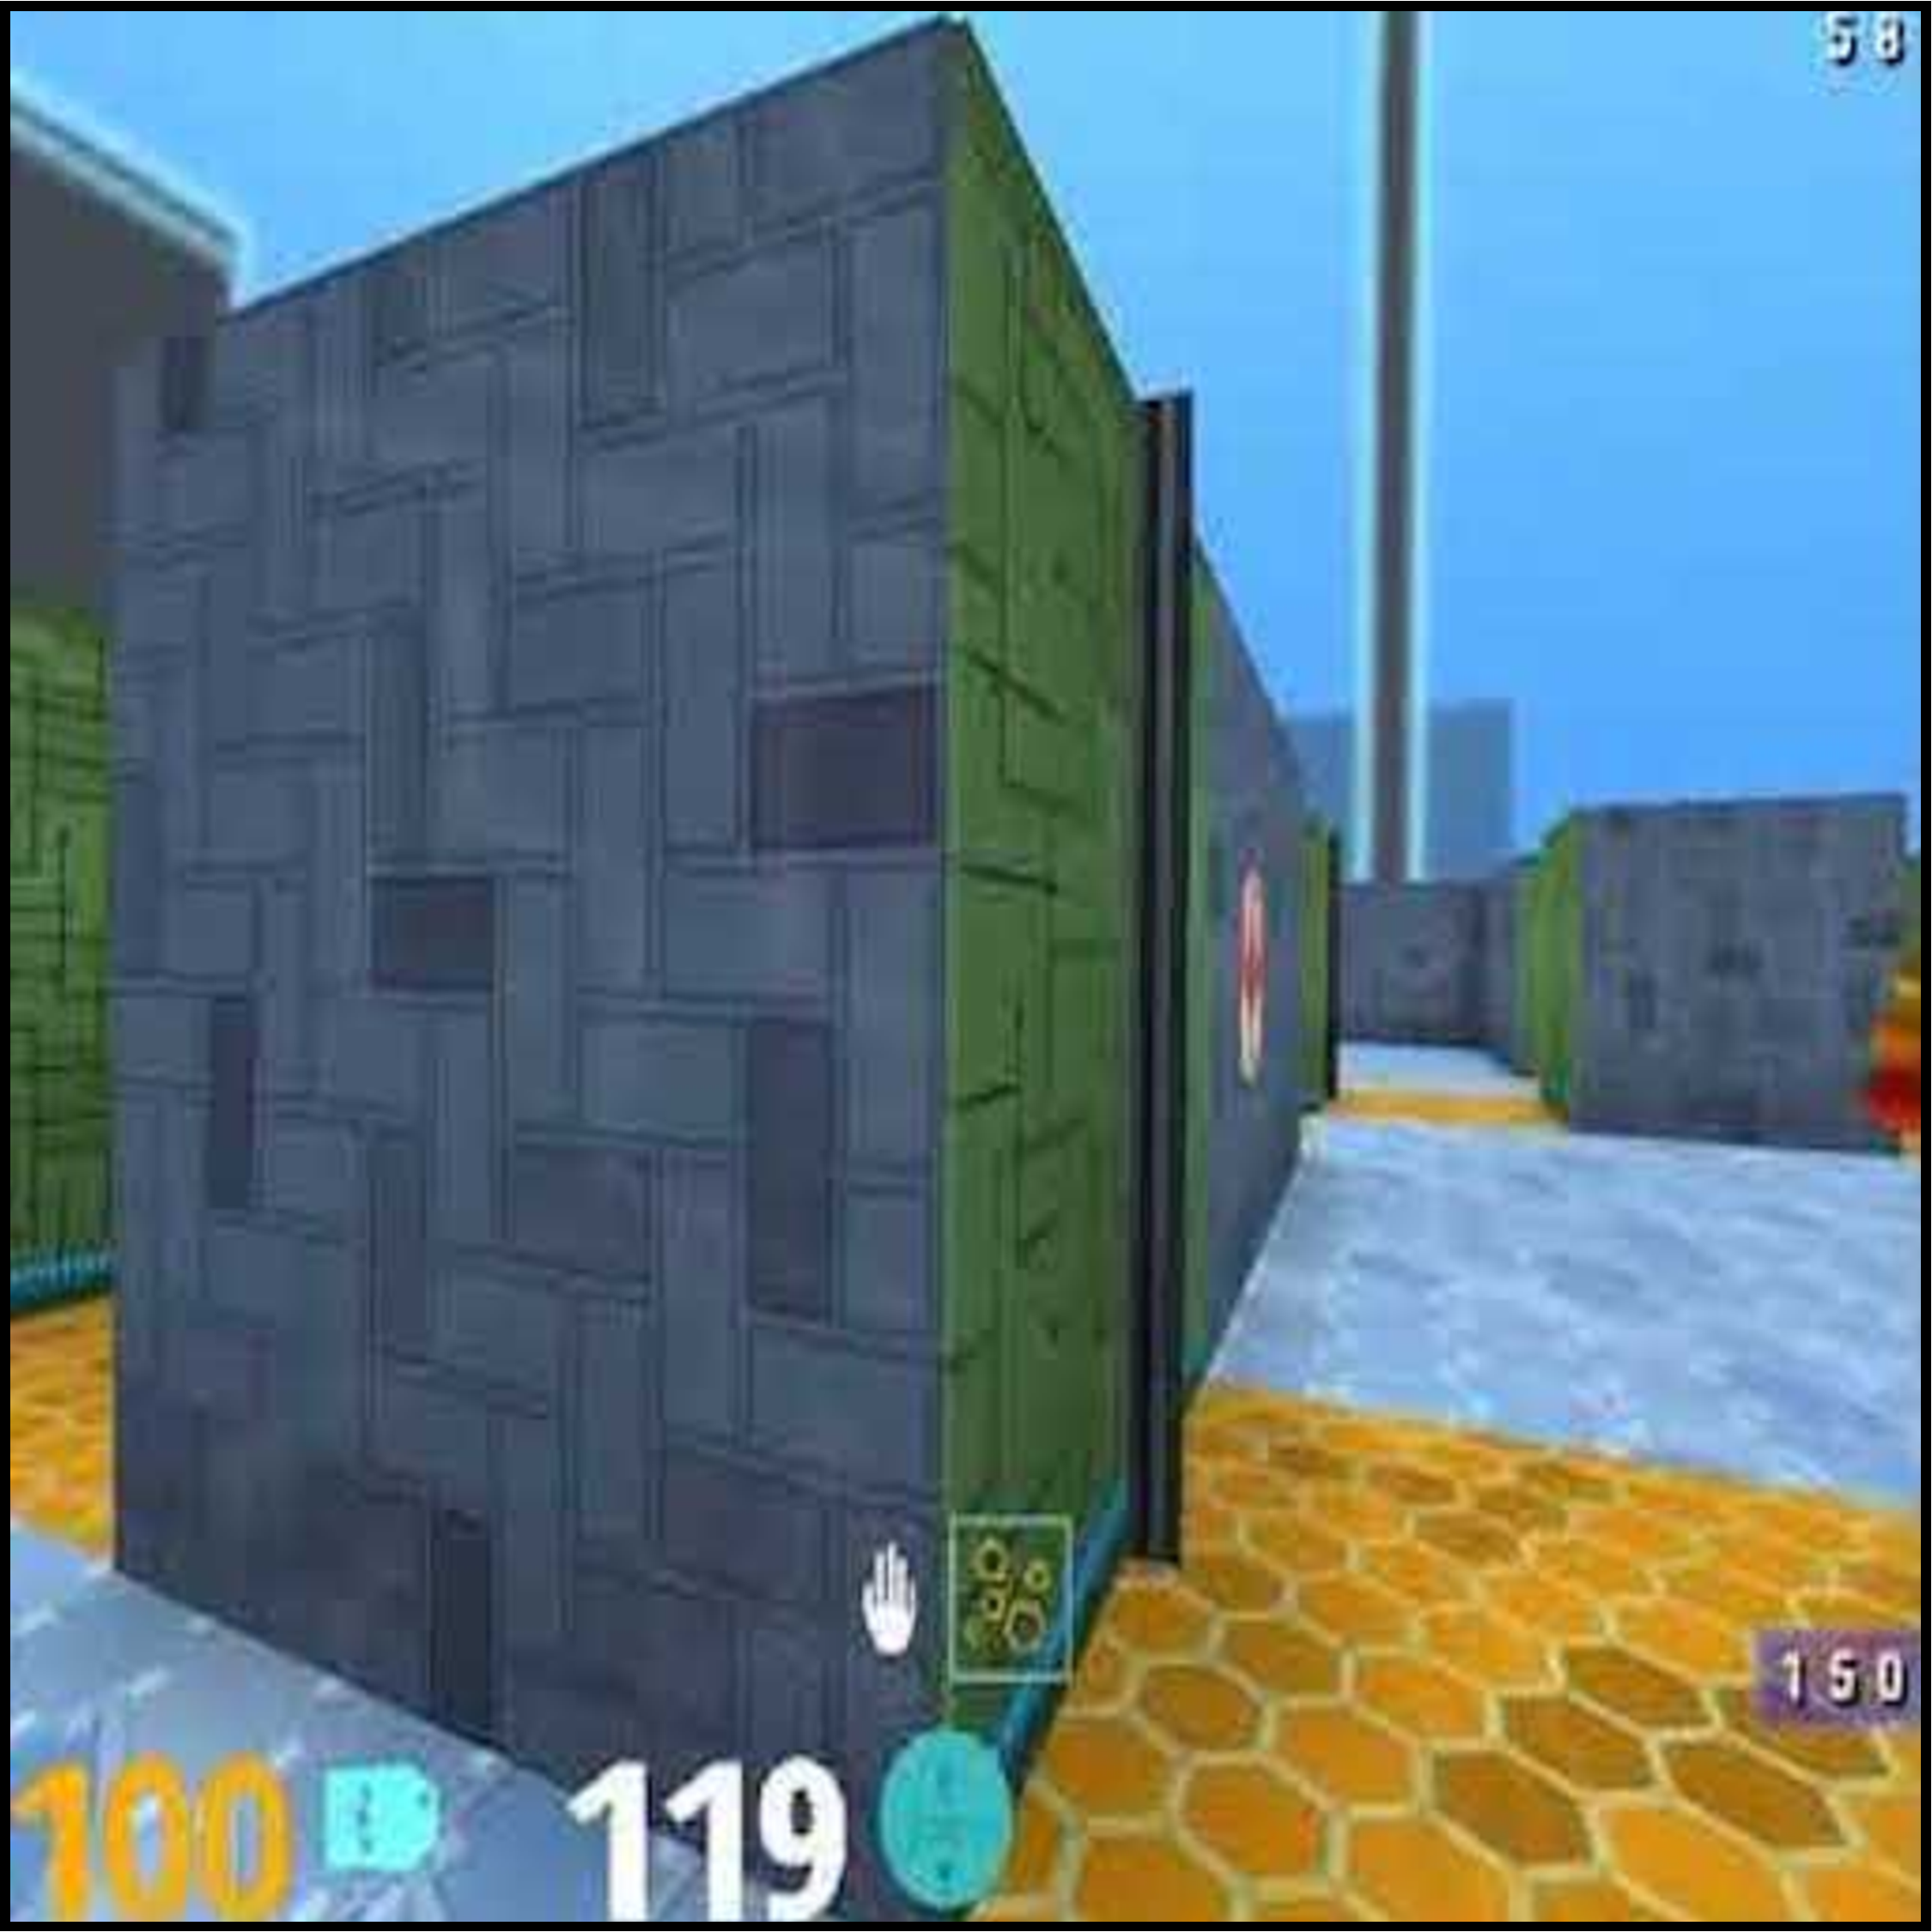
\includegraphics[width=\textwidth]{fig/tasks/goal_maze.pdf}
        \caption{Goal Maze}
        \label{fig:tasks:goal_maze}
    \end{subfigure} 
    \hfill
    \begin{subfigure}[t]{0.19\textwidth}
        \centering
        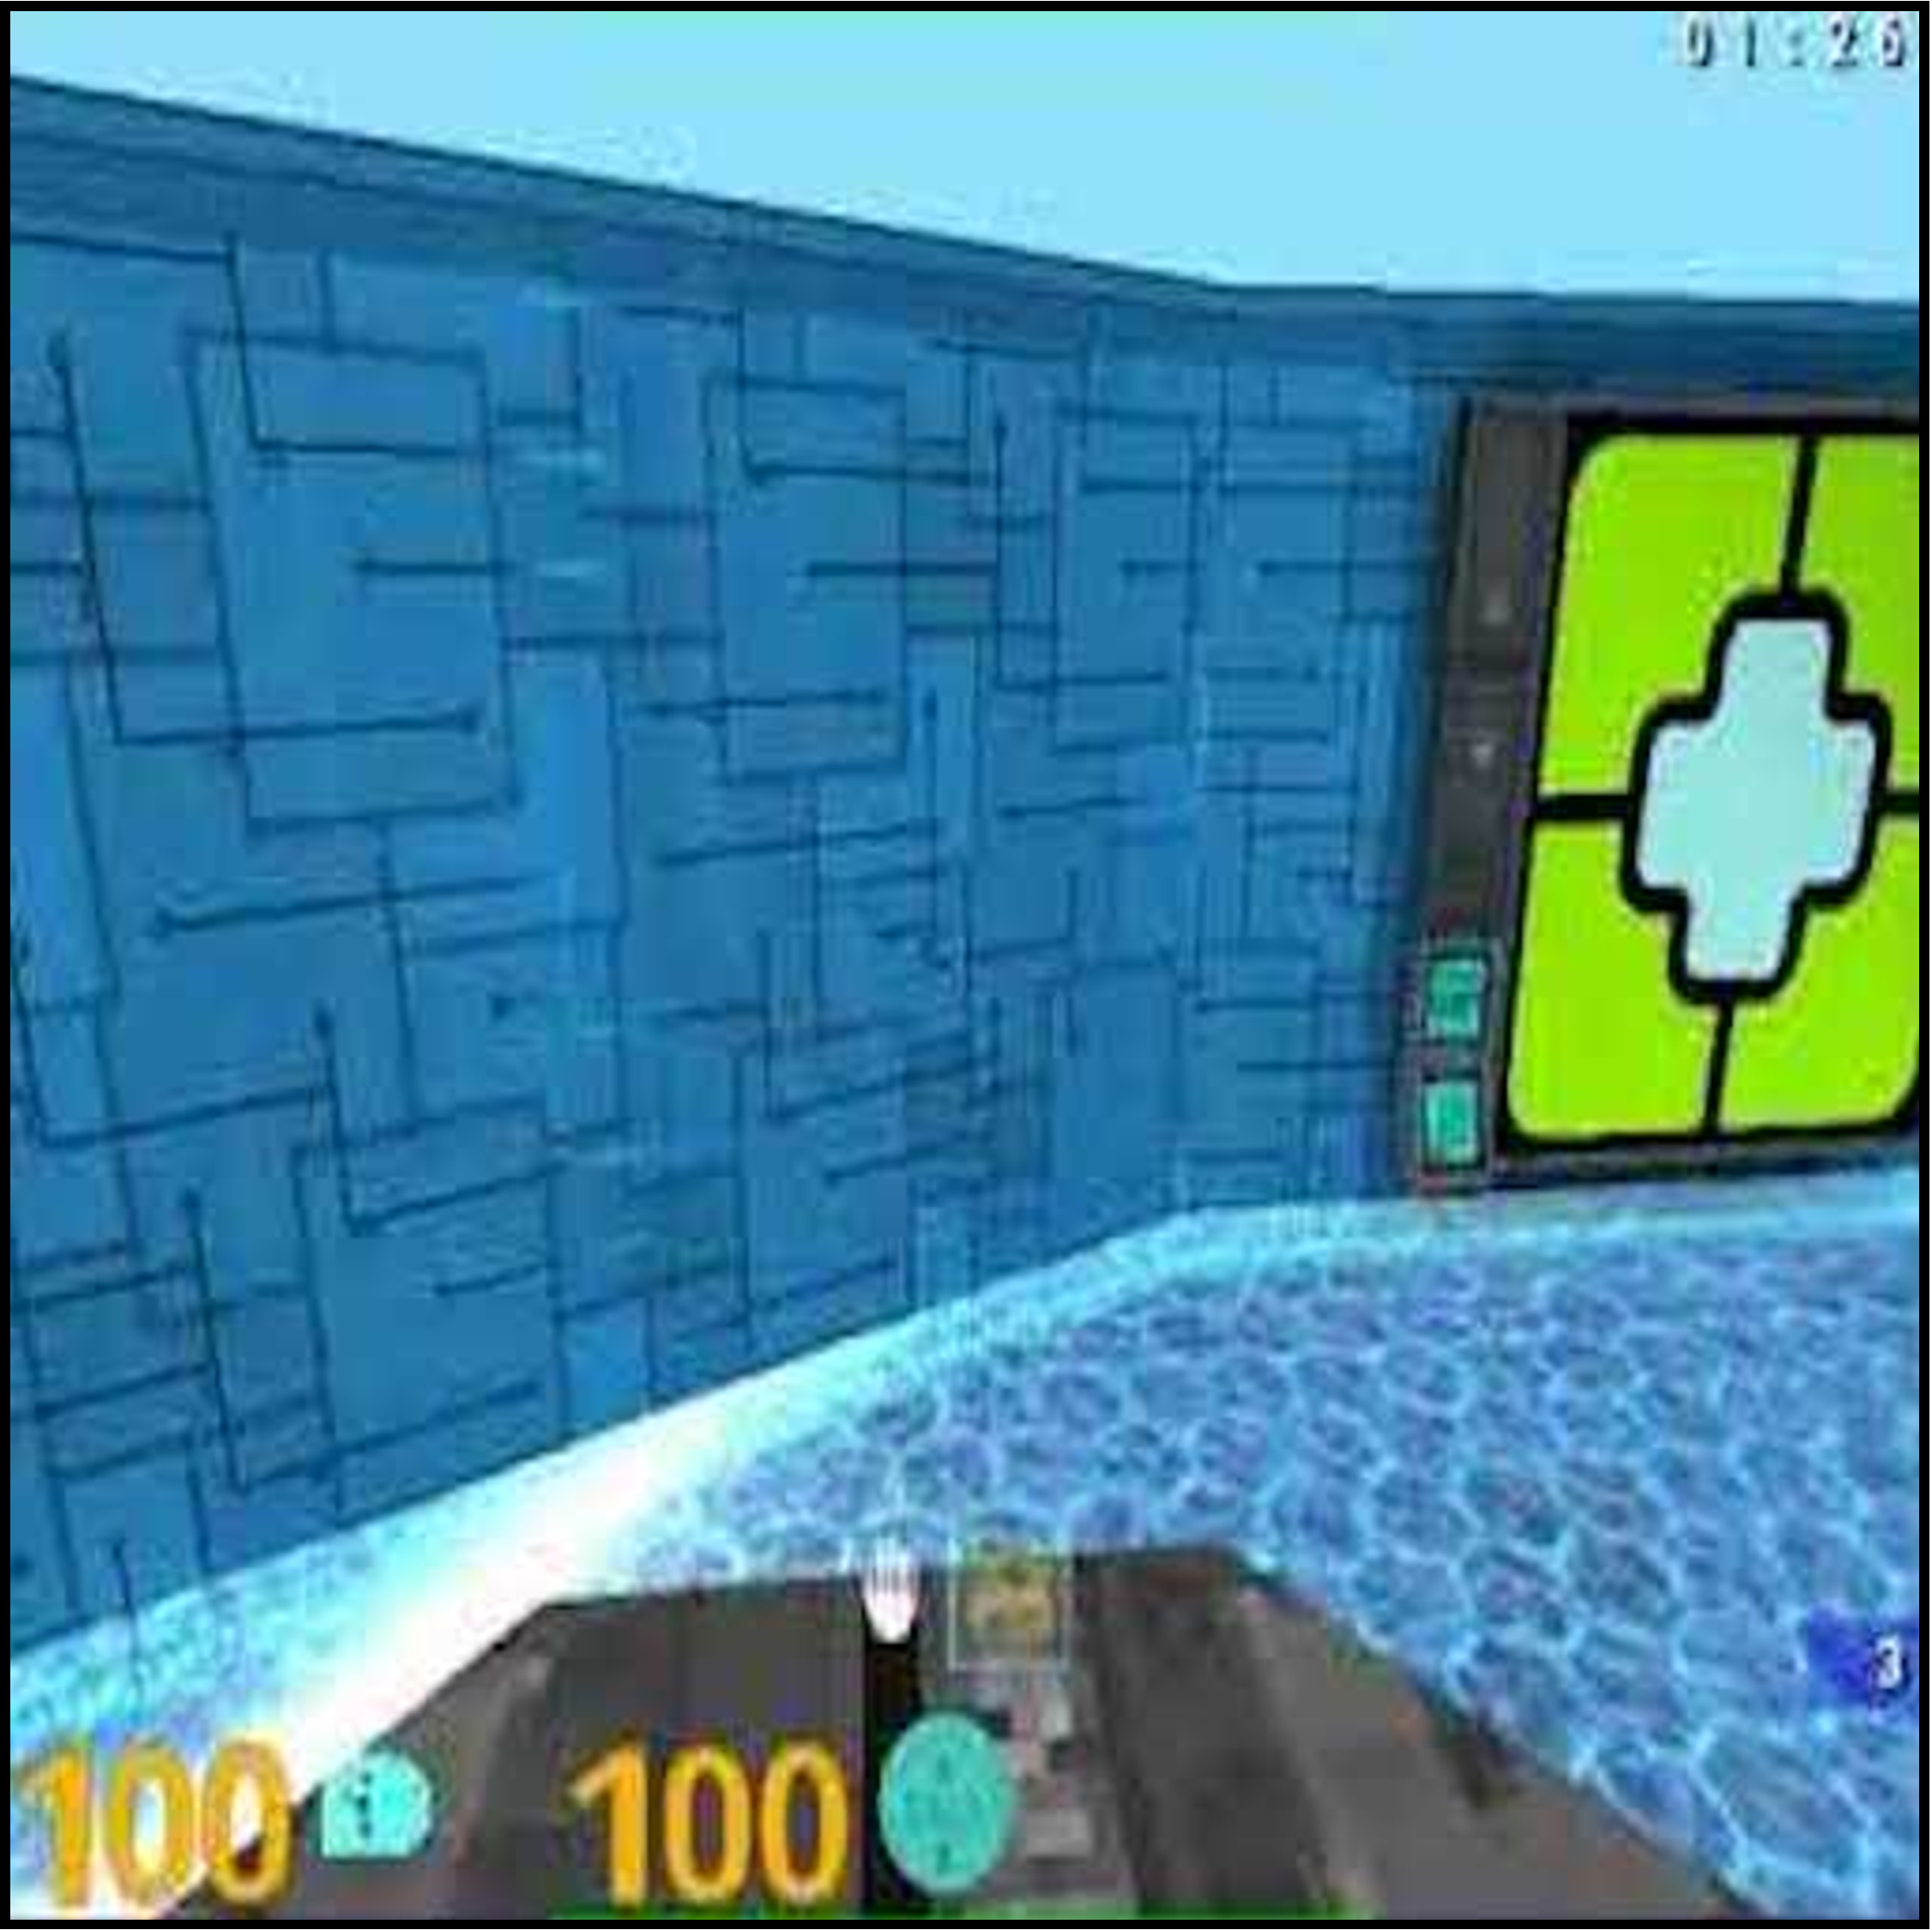
\includegraphics[width=\textwidth]{fig/tasks/watermaze.pdf}
        \caption{Watermaze}
        \label{fig:tasks:watermaze}
    \end{subfigure}
    \hfill
    \begin{subfigure}[t]{0.19\linewidth}
        \centering
        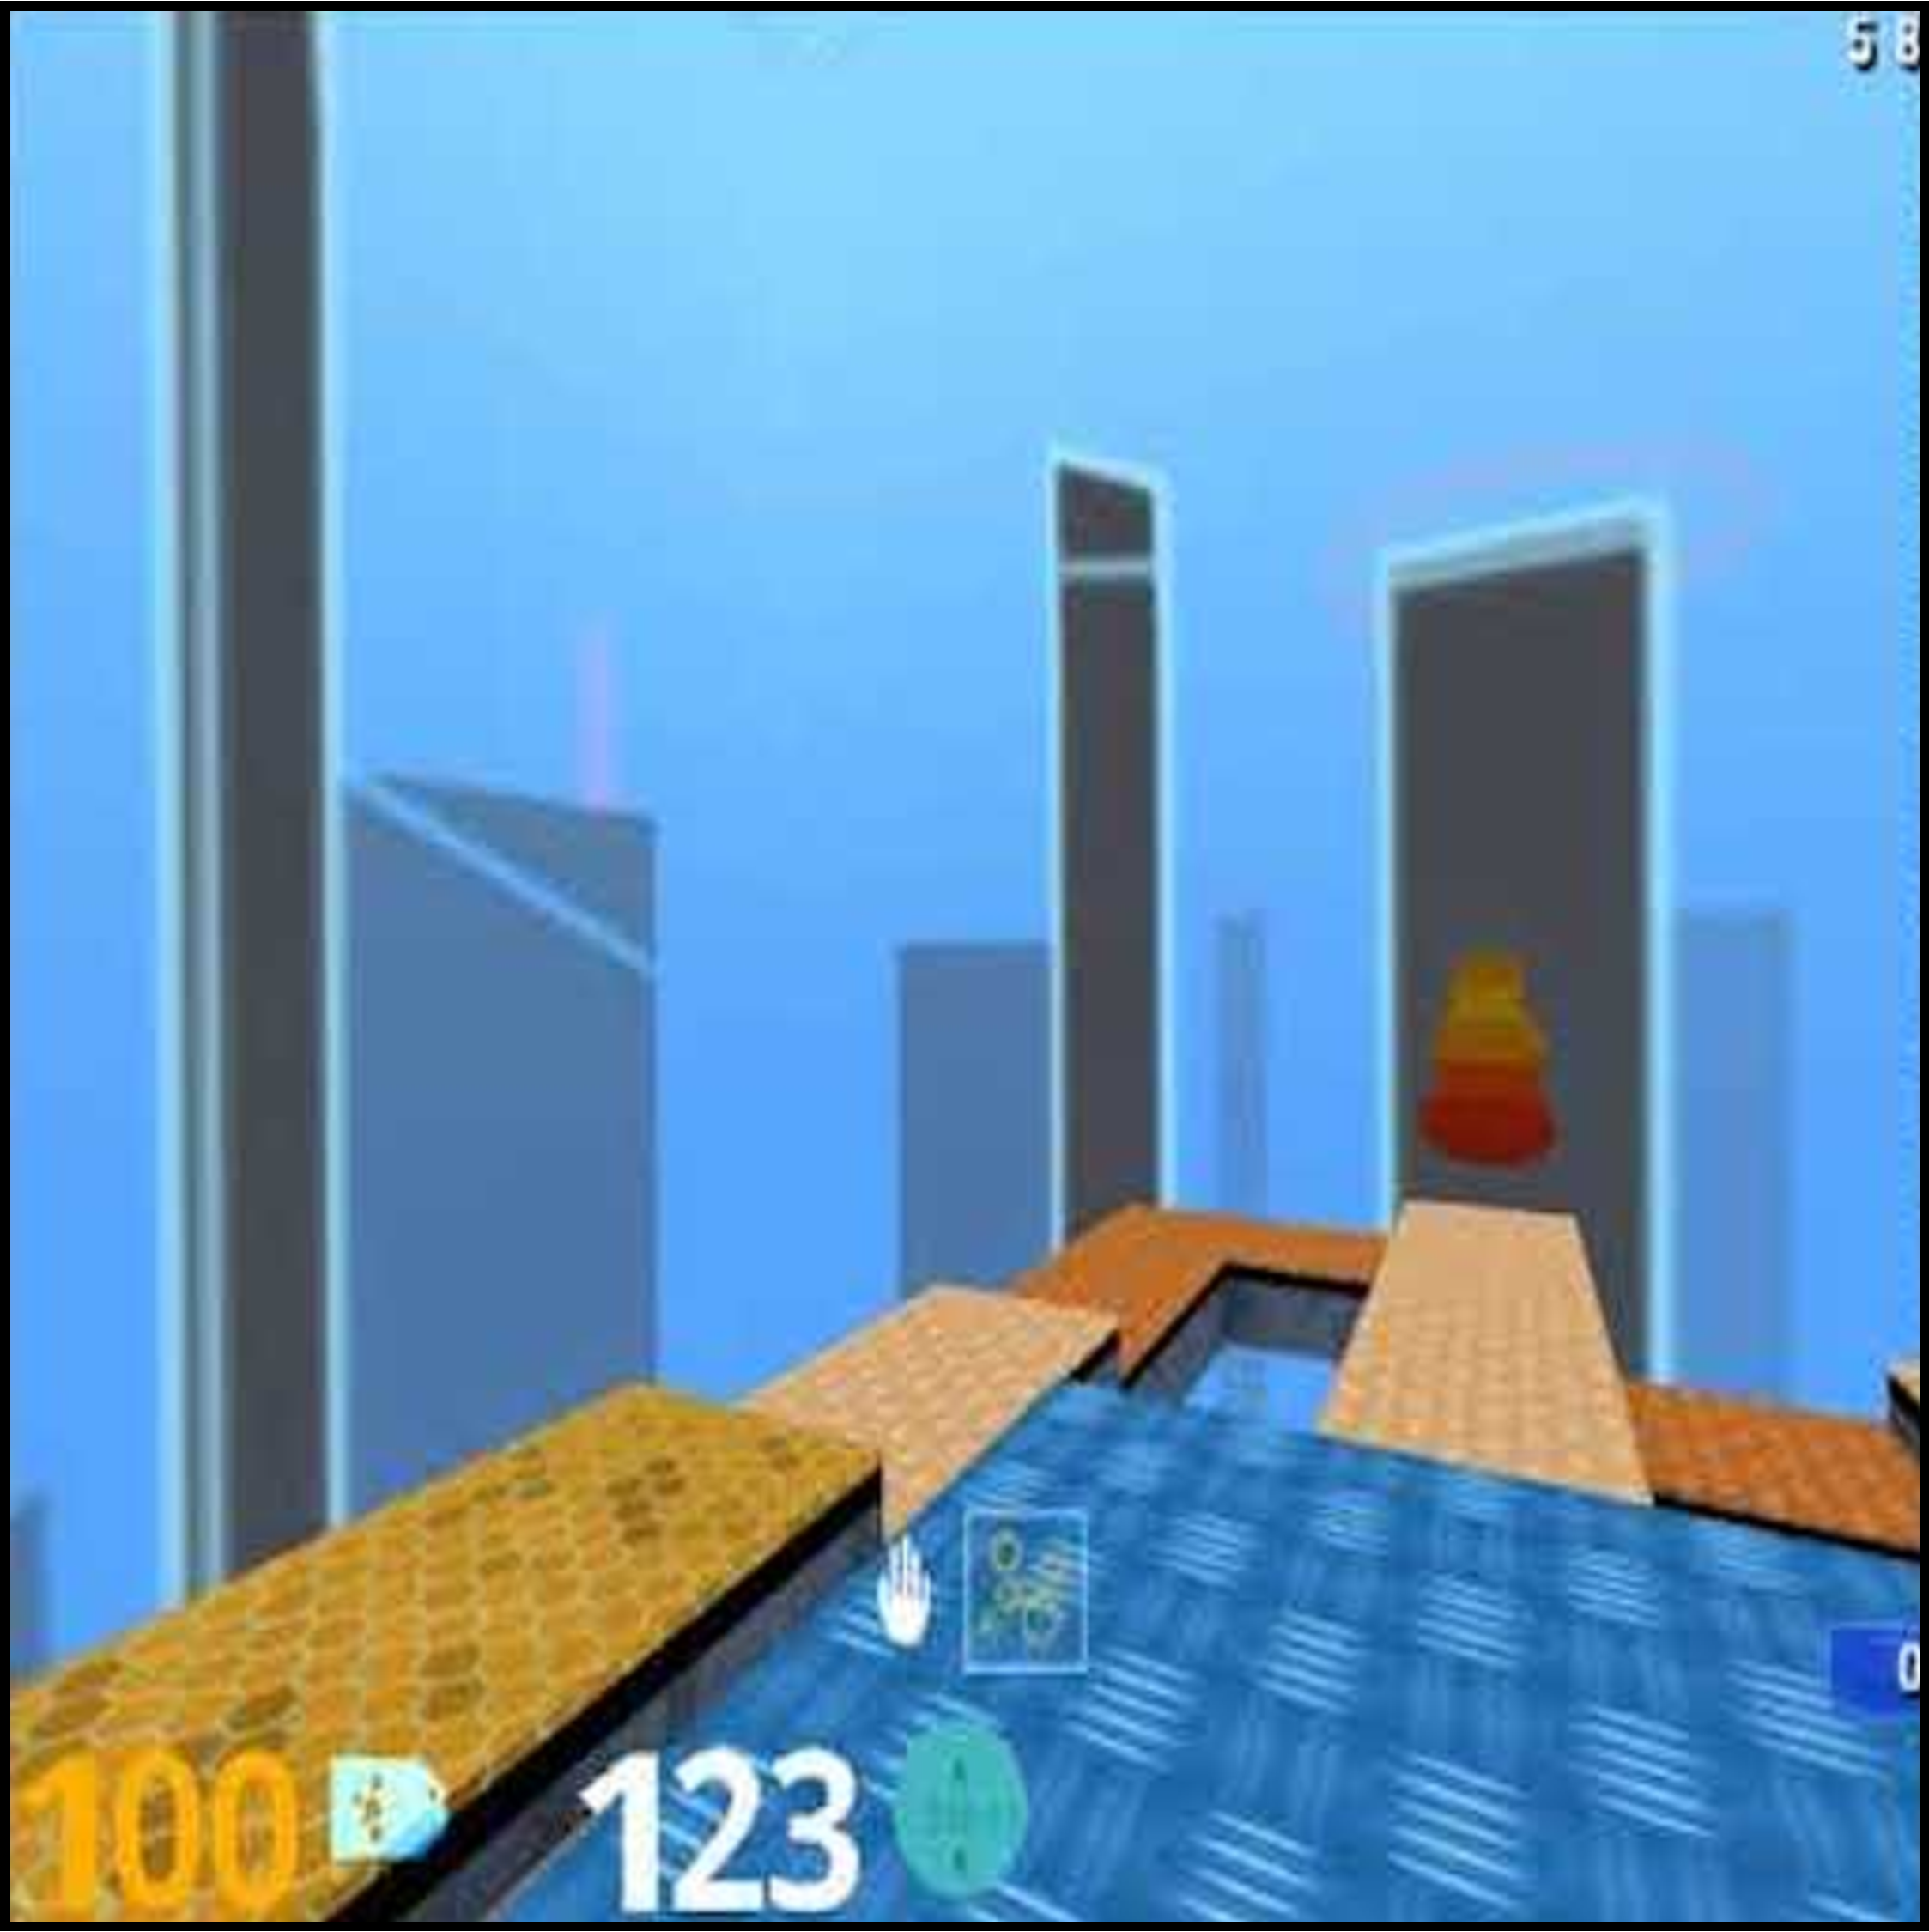
\includegraphics[width=\linewidth]{fig/tasks/irreversible_path.pdf}
        \caption{Irreversible Path}
        \label{fig:tasks:irreversible_path}
    \end{subfigure}
    \hfill
    \begin{subfigure}[t]{0.19\linewidth}
        \centering
        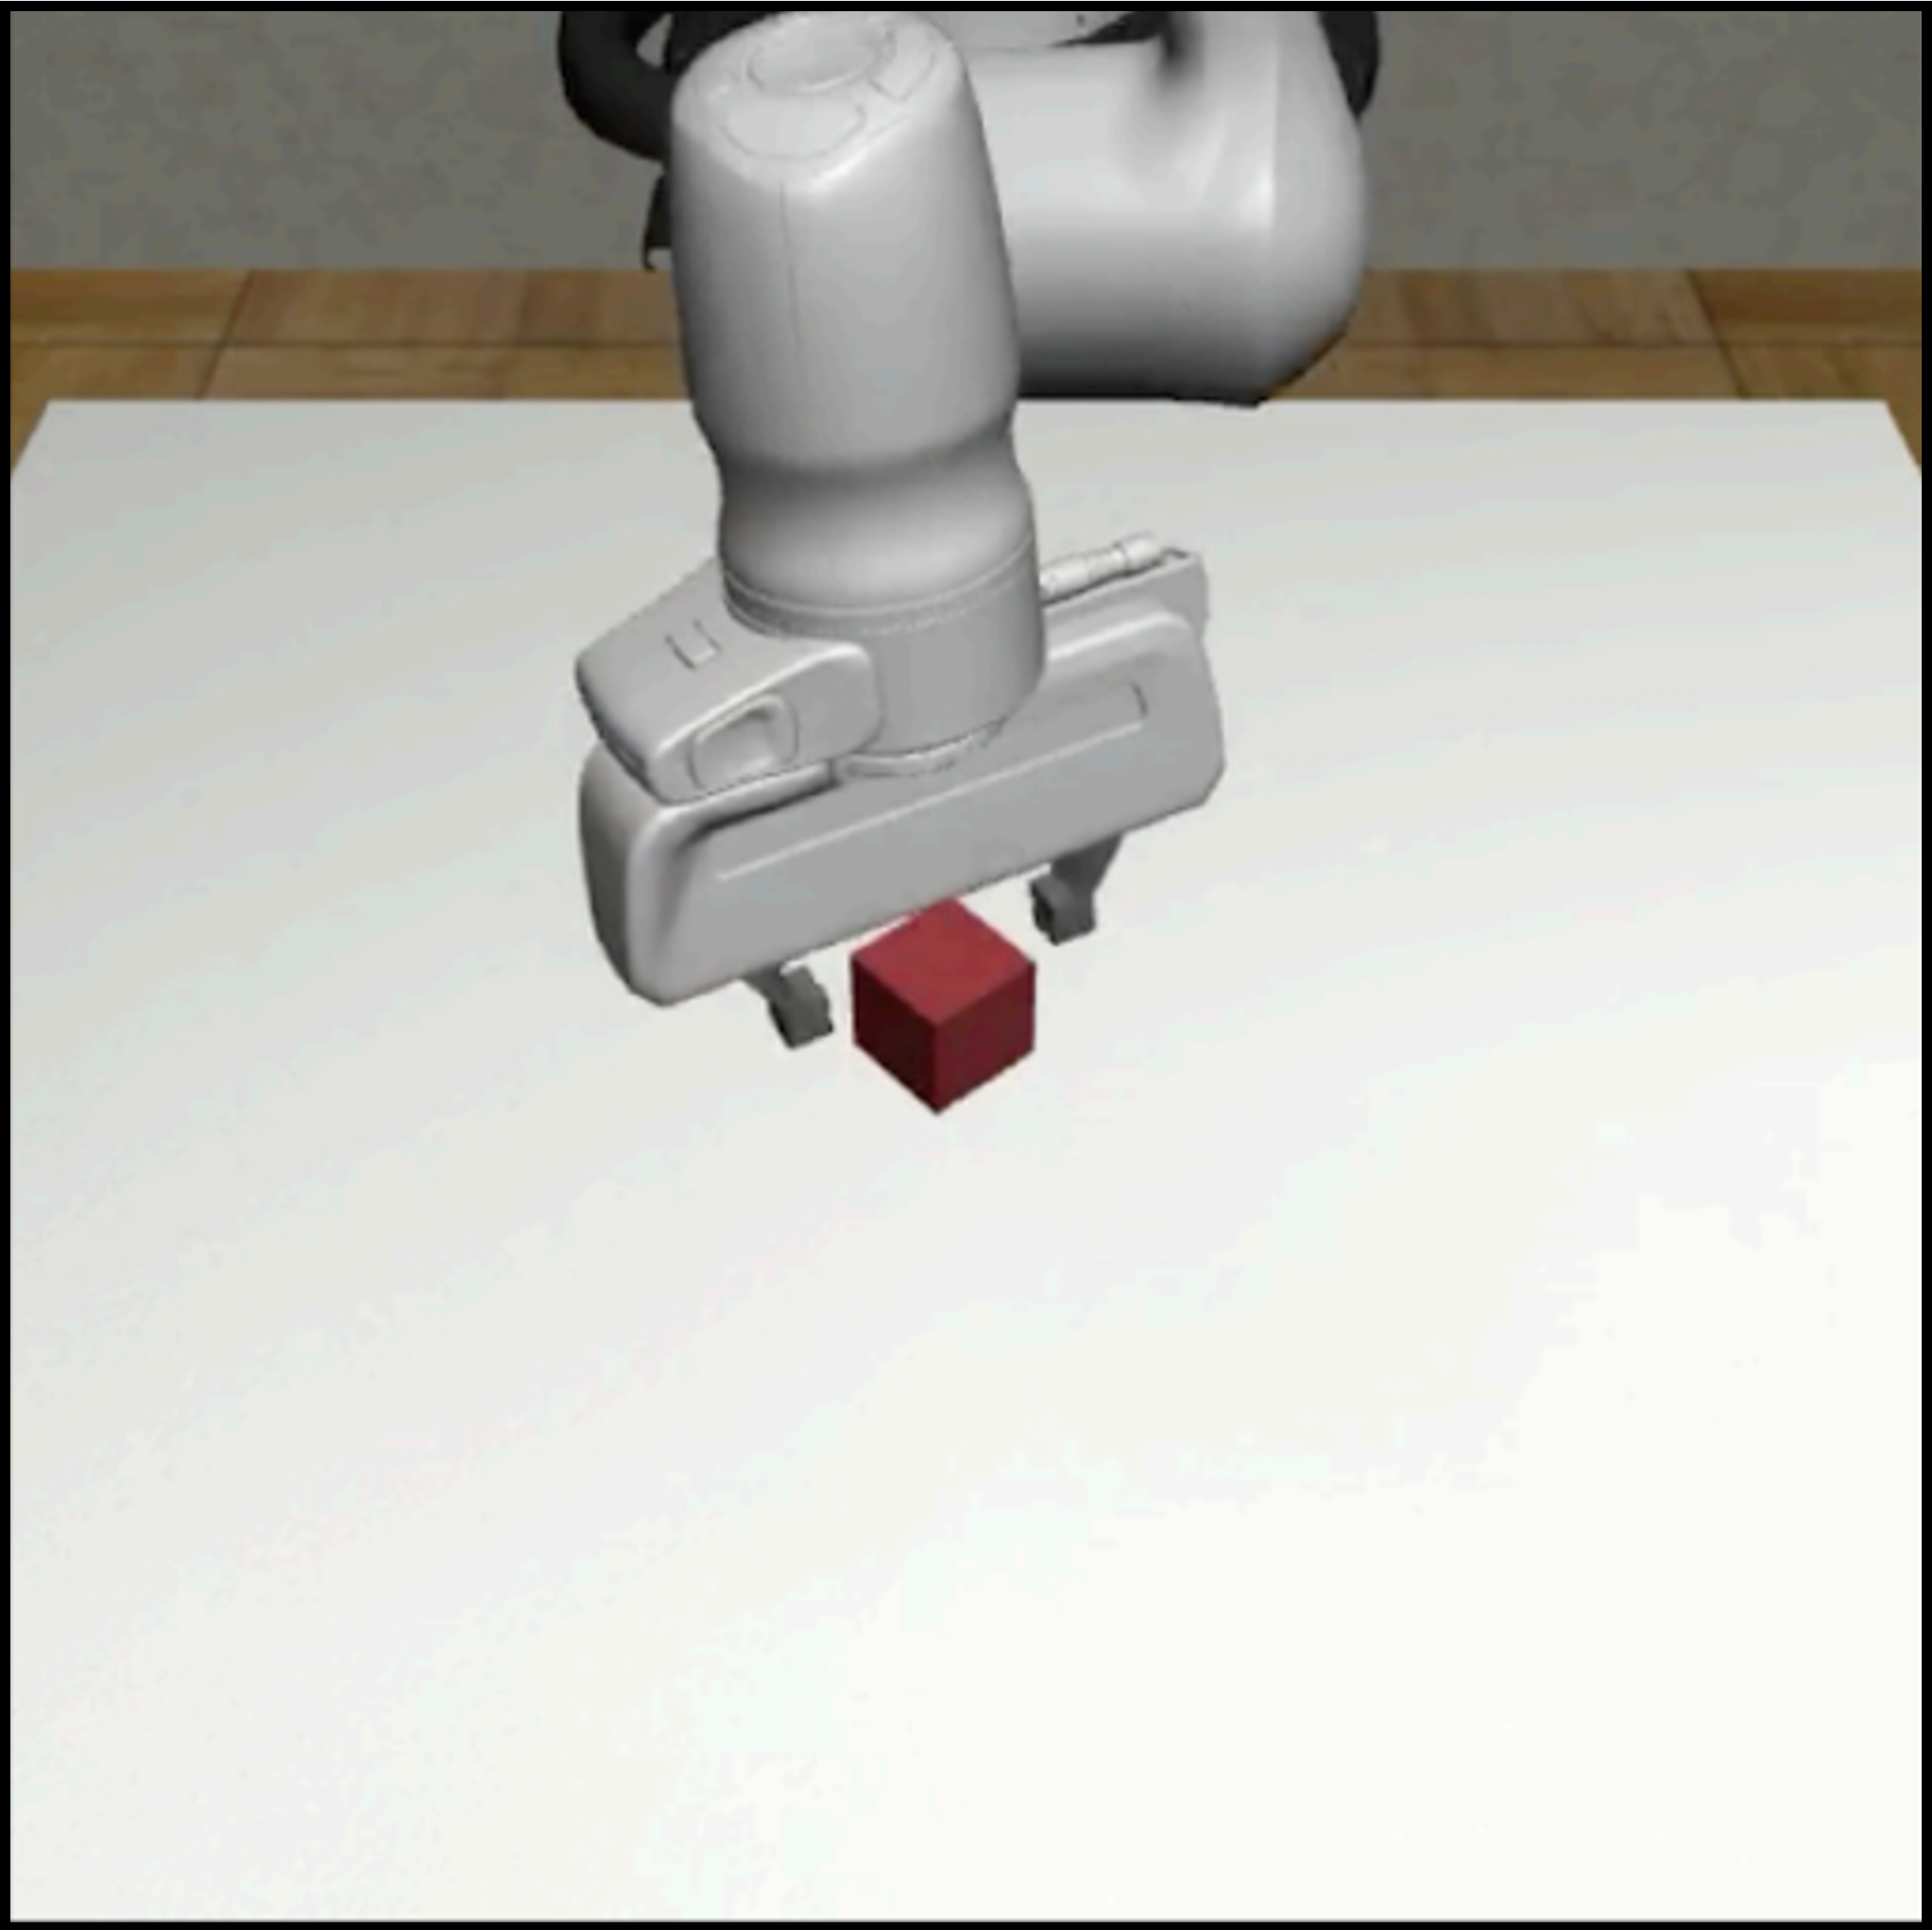
\includegraphics[width=\linewidth]{fig/tasks/lift.pdf}
        \caption{Lift}
        \label{fig:tasks:lift}
    \end{subfigure} 
    \hfill
    \begin{subfigure}[t]{0.19\linewidth}
        \centering
        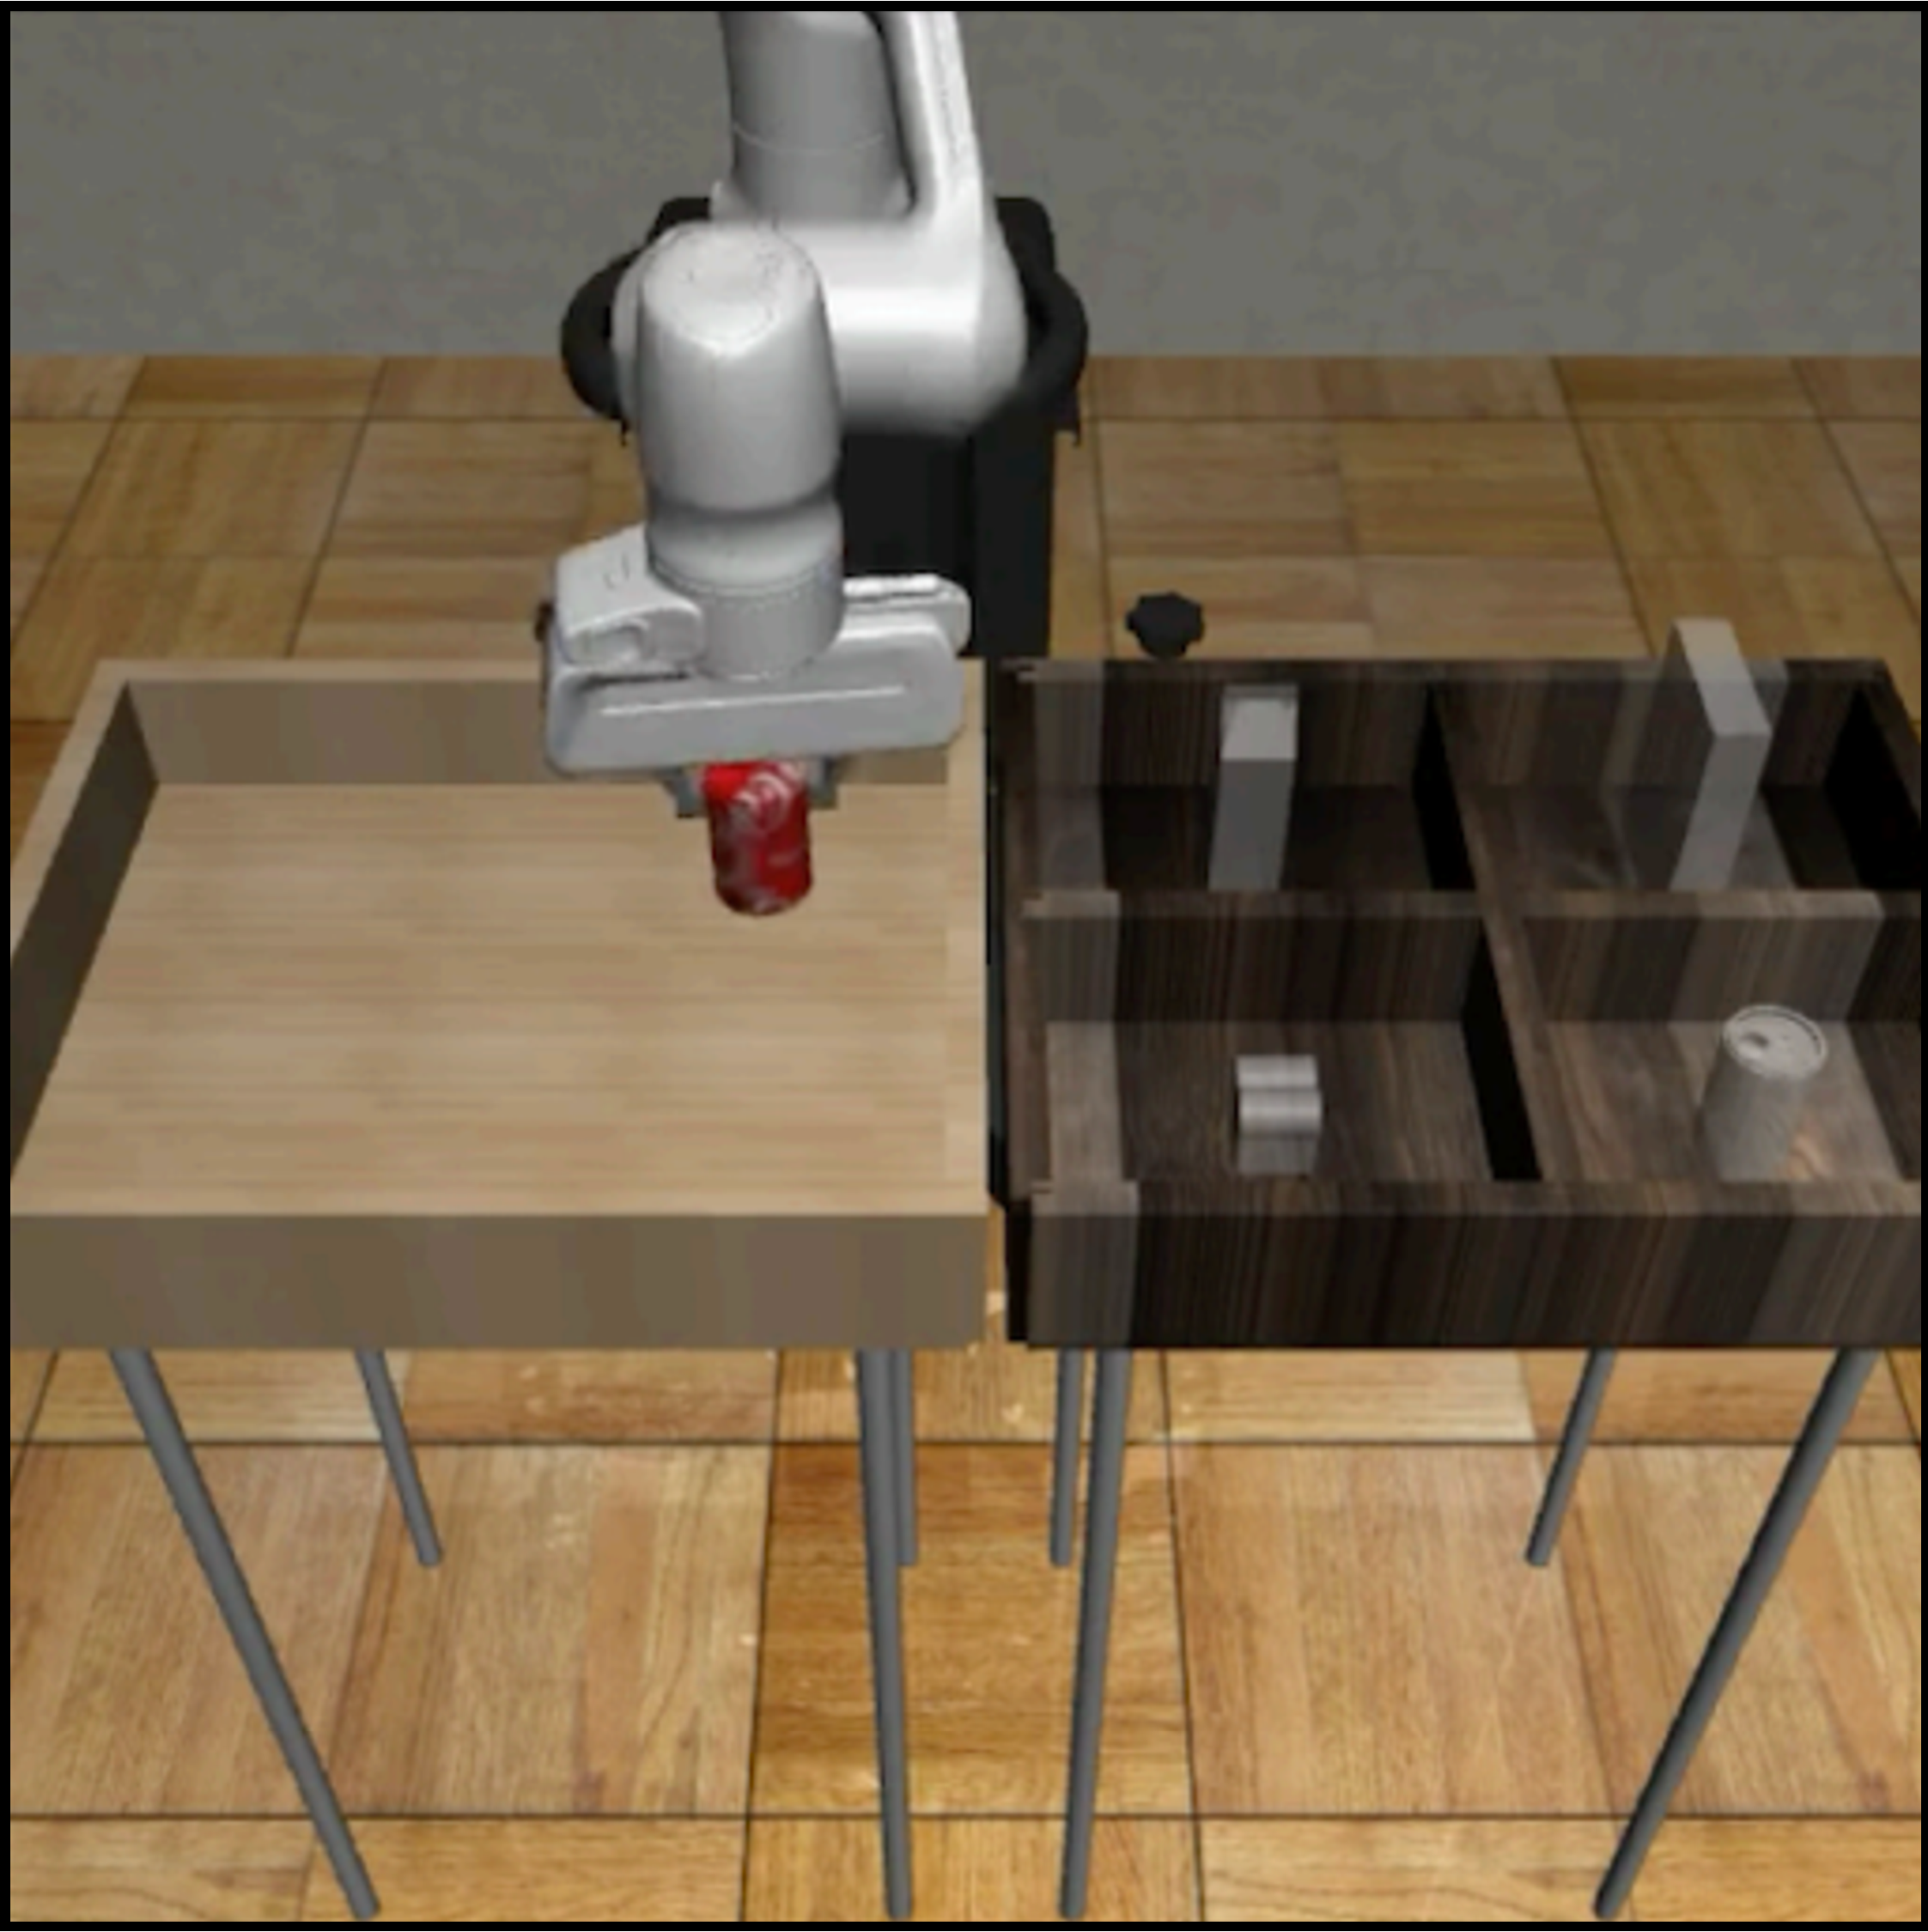
\includegraphics[width=\linewidth]{fig/tasks/can.pdf}
        \caption{Can}
        \label{fig:tasks:can}
    \end{subfigure} 
    \caption{
        We evaluate our method on five tasks that cover challenges such as exploration and planning over long horizons in RL settings, as well as object manipulation and continuous control in IL settings.
        Figures are from \citet{beattie2016deepmind} and \citet{mandlekar2021matters}.
    }
    \label{fig:tasks}
  \vspace{-1em}
\end{figure}